\documentclass[a4paper, 11pt, titlepage]{jsarticle}
\usepackage[dvipdfmx]{graphicx}
\usepackage{amsmath}
\usepackage{listings}

\title {知能情報実験1 : レポート課題1}
\author{205713B  朝比奈 太郎}
\date{\today }

\begin{document}
\maketitle
\tableofcontents
\clearpage

\section{はじめに}
\subsection{講義の目標と達成目標}

知能情報実験の目的は,知能情報工学分野の知識や技術について,座学で学んだ内容を実践することによって理解を深め,今後の専門科目の学習の基礎を築くことである.具体的には,論理回路やプログラムの作成に関する実習およびレポート作成を通して,その背景にある知識を体系的に理解し,使えるようになることを目指す.

知能情報実験におけるレポート作成には\TeX を利用する。
\cite{okumura,texwiki,texshop,mactex,texcom}. \TeX による文書作成技術は,理工系の学術資料作成の標準技術である.これを学ぶことによって卒業研究における報告書や論文の作成,大学院での研究における学術論文の作成の基礎技術を習得する.
具体的には,以下の7つの技術の習得を目指す.

\begin{enumerate}
\item \TeX 文書の基本構成の理解,組版
\item 特殊文字表記,文字装飾,箇条書き
\item 表組,図表・ソースコードの挿入・参照
\item 基礎的な数式表記
\item 参考文献リストの作成、参照
\end{enumerate}

\subsection{\TeX (テフ,テック)とは}
\TeX とは,テキストや図などを紙面に構成する組版(くみはん)システムである.\TeX には以下のような特徴がある.

\begin{itemize}
\item フリーソフト
\item 多彩なOSで利用可能 (windows, mac, Linux, etc)
\item テキストエディタで読み書き可能
\item 自動ハイフネーションやペアカーニングなどの高度な組版技術
\item 相互参照(参考文献, 図表番号)の自動割り当て技術
\item 数式組版:数式をテキスト形式で表す標準型
\end{itemize}

\section{\TeX によるレポート作成技術}
\subsection{改行と改ページ}
\subsubsection{改行}
\TeX 文書における改行方法は主に2つある.1つ目は空行を入れる方法である.この段落後に空行を入れることで文章が改行され,次行の文頭には自動的にインデント処理が施される.

2つ目は,バックスラッシュを2つ続きで記述する方法である.この段落後にバックスラッシュを2つ続きで記述することで文章が改行される.しかし,空行による改行とは異なり,次行の文頭のインデント処理は行われない.\\
したがって,これら2つの方法はどちらも改行処理であるが,全く同一の処理ではないので使用の目的により使い分ける必要がある.標準的には空行による方法を用いると良い.

\subsubsection{改ページ}
\TeX ファイル内で改ページを行う方法は主に2つある.1つ目はnewpage命令による方法である.この段落の後にnewpage命令を実行すると,命令後の文章からは新しいページに記載される.newpage命令以前に命令した図表で配置が決まっていないものがあっても,本文だけが改ページされる.
\newpage

2つ目はclearpage命令による方法である.この段落の後にclearpage命令を実行すると,命令後の文章からは新しいページに記載される.clearpage命令以前に命令した図表で配置が決まっていないものがあれば,それらを配置した後に改ページが実行される.
\clearpage

\subsection{特殊記号表記および文字装飾}
\subsubsection{特殊記号}
数式表現や\TeX の命令記号を本文中で表示する場合は,各記号の前にバックスラッシュを付する.例えば,アンダーバー(\_),ドルマーク(\$),アンド(\&),括弧(\{,\}),半角スペース(\ ),パーセント(\%),シャープ(\#)などである.バックスラッシュ(\textbackslash )を表記したい場合には,textbackslashという文字列の前にバックスラッシュを付ける.

\subsubsection{文字装飾}
文字装飾には文字装飾命令を使用する.例えば,太字は「\textbackslash textbf{\ }」,下線は「\textbackslash underline{\ }」,斜体は「\textbackslash textit{\ }」である.この命令記述の{\ }内に装飾したい文字列を記述する.実際にこれらの命令を使用して文字を装飾すると次のようになる: \textbf{琉球大学}, \underline{琉球大学}, \textit{University of the Ryukyus}.

\subsection{表組および表の挿入方法}
\begin{table}[htbp]
\caption{基本的な文字装飾の方法}
\label{tabel1}
       \centering
	\begin{tabular}{|c||l|}
           \hline
           種類 & 実行例\\
           \hline
           \hline
           太字 & \textbf{琉球大学}\\
           \hline
           下線        & \underline{琉球大学}\\
           \hline
           イタリック    & \textit{University of the Ryukyus}\\
           \hline
       \end{tabular}
\end{table}
     
\subsection{図の挿入方法}
\TeX 文書に図を挿入するためにはfigure環境を用いる.figure環境内で,includegraphics命令を用いて図を挿入する.一般的なレポート作成では,図題(図タイトル)をcaption命令により図の下部に付記する.また,本文中での図番号参照のためにlabel命令を用いて図に固有の名前を与える.

\subsection{ソースコードの挿入方法}
\TeX ファイルにソースコードを挿入するためにはlstinputlisting命令を使用する.この命令を使用するためには,listingsパッケージをインクルードする必要がある.これらの環境を用いることで, Listing \ref{pg:sample}ソースコード内の特殊記号やインデントなどをソースファイルに記述されたとおりに表示できる.

\begin{figure}[htbp]
    \centering
    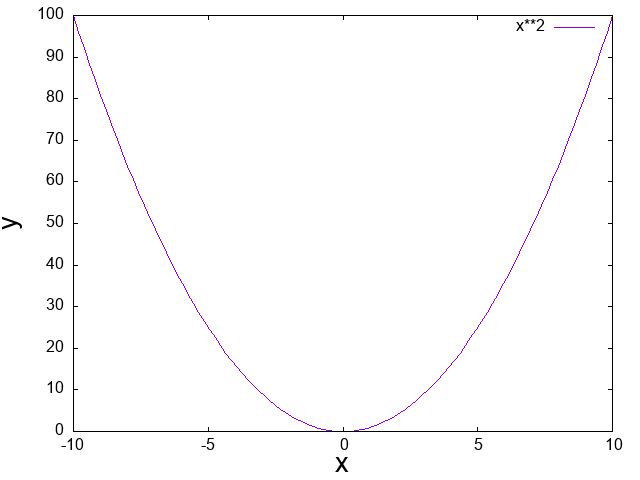
\includegraphics[width=120mm]{graph.png}
    \caption{二次関数}
    \label{fig1}
\end{figure}
\newpage


\lstinputlisting[language=Python, numbers=left, breaklines=true, basicstyle=\ttfamily\footnotesize, frame=single, caption=サンプルプログラム, 
label=pg:sample]{sample.py}

\subsection{数式表現の基礎}
\subsubsection{本文中の数式やギリシャ文字の表示}
本文中に数式を表示したい場合には数式を\$で囲む.具体的には\$y=ax+b\$と記述すると,$y=ax+b$と出力される.この方法によってギリシャ文字($\alpha $, $\beta $, $\delta $, $\epsilon $, $\theta $, $\lambda $, $\mu $, $\pi $, $\tau $, $\phi $など)も表記することができる.
 
\subsubsection{数式表示}
数式は,以下のように独立した行に記述することもできる.
\[
\sum _{i=0}^{2} x_i^2 = x_0^2+x_1^2+x_2^2.
\]

さらに,以下の式(\ref{eq0})$\sim $(\ref{eq2})のように,数式番号をつけることもできる.
\begin{align}
y &= ax+b, \label{eq0}\\
\frac{dx}{dt} &=a_{11}x+a{12}y, \label{eq1}\\
\frac{dy}{dt} &=a_{21}x+a{22}y, \label{eq2}
\end{align}

式(\ref{eq1})$\sim $(\ref{eq2})を行列形式で簡略化して,以下の式(\ref{eq3})のように記述することもできる.

\begin{align}
    \left(    \begin{array}{c}
                    \dot{x} \\
                    \dot{y}
                \end{array} \right)
    =
    \left(    \begin{array}{cc}
                   a_{11} & a_{12} \\
                   a_{21} & a_{22}
               \end{array} \right)
    \left(    \begin{array}{c}
                   x \\
                   y
               \end{array} \right)    . \label{eq3}
\end{align}

\section{演習問題 A}
表2は,野菜の価格を示している.
\begin{table}[htbp]
\caption{野菜の価格}
\label{tabel1}
       \centering
	\begin{tabular}{|l| |c|r|c|}
           \hline
           種類 & 販売単位 & 価格 & 割引\\
           \hline
           キャベツ & 1/4個& 78円& \textbf{30\%引き}\\
           にんじん & 2本& 158円& \\
           舞茸& 100g& 138円& 10\%引き\\
           \hline
       \end{tabular}
\end{table}

\section{演習問題B}
gnuplotで以下のコマンドを入力すると,作業ディレクトリ下に"gnu\_sample.png"という名前の画像ファイルが生成される.

\begin{enumerate}
\item gnuplot
\item gnuplot \textgreater \ set term png enhanced size 640, 480
\item gnuplot \textgreater \ set output "gnu\_sample.png"   
\item gnuplot \textgreater \ plot sin(x) title "y = sin(x)" with lines lw 3
\end{enumerate}

\section {演習問題 C}
期待値と分散はそれぞれ以下の式(\ref{eq4}),(\ref{eq5})で記述できる.\\

\begin{align}
&E[X] = \mu = \sum _i p_i x_i \label{eq4}\\
&V[X] = \sigma^2 = E[(X - E[X])^2] = \sum _i (x_i - \mu)^2 p_i \label{eq5}
\end{align}

正規分布は, 平均値を$\mu $, 標準偏差$\sigma $をとすると, 以下の式で記述できる.\\
\[
f(x) = \frac{1}{\sqrt{2 \pi \sigma}} \exp{( - \frac{(x - \mu)^2}{2 \sigma ^2})}
\]
\section{演習問題 D}
図2は, $y=2x^3+2x^2+x-1$と$y=3sin(2x)-1$ のグラフを示している.

\begin{figure}[htbp]
    \centering
    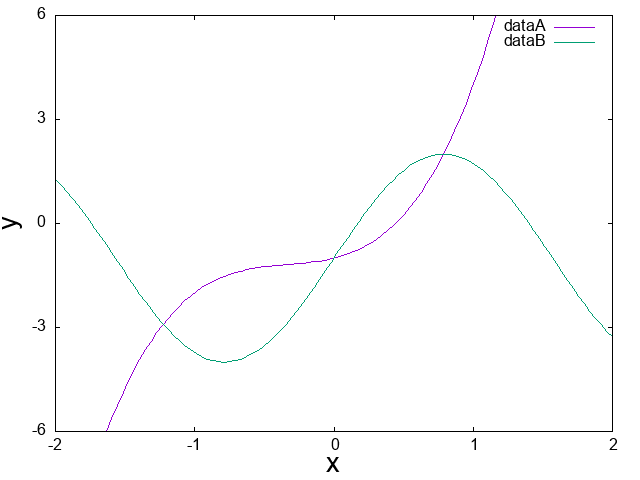
\includegraphics[width=120mm]{graph2.png}
    \caption{三次関数と三角関数}
    \label{fig2}
\end{figure}


\begin{thebibliography}{99}
\bibitem{okumura} 奥村晴彦, 黒木祐介, \LaTeX 2e美文書作成入門(改訂第6版),技術評論社, 2013,
\bibitem{texwiki} TEX WIKI, https://texwiki.texjp.org/, 2018/03/24.
\bibitem{texshop} TeXShop, http://pages.uoregon.edu/koch/texshop/, 2018/03/24.
\bibitem{mactex} MacTeX, http://tug.org/mactex/, 2018/03/24.
\bibitem{texcom} LaTeXコマンド集, http://www.latex-cmd.com/, 2018/03/24.
\end{thebibliography}

\end{document}